\documentclass[a4paper, 12pt]{report}

\usepackage{charter}
\usepackage{makeidx}
\usepackage{fancyhdr}
\usepackage{hyperref}
\usepackage[utf8]{inputenc}
\usepackage{graphicx}
\usepackage[left=2cm, right=2cm]{geometry}
\usepackage{latexsym}
\usepackage{amsmath, amsthm, amssymb}
\usepackage{rotating}


\begin{titlepage}
\title{Documento di Analisi}
\author{Release 1.4}
\date{\today \\Firenze \\\begin{figure}[h] \centering

\includegraphics[width=0.2\textwidth]{../../images/logokiwi.png} \end{figure} }
\end{titlepage}

\pagestyle{fancy}

\begin{document}

\maketitle

\section*{Approvazione, redazione, lista distribuzione}
\begin{table}[h!]
  \begin{center}
    \begin{tabular}{| l | l | p{60mm} |}
    \hline
    \textbf{approvato da} & \textbf{il giorno} & \textbf{firma} \\
	\hline    
	Marco Tinacci & \today &  \\
    \hline
    \end{tabular}
  \end{center}
\end{table}

\begin{table}[h!]
  \begin{center}
    \begin{tabular}{| l | l | p{60mm} |}
    \hline
    \textbf{redatto da} & \textbf{il giorno} & \textbf{firma} \\
    \hline
    Francesco Calabri & \today &  \\
    \hline
	Manuele Paulantonio & \today &  \\
    \hline    
	Massimo Nocentini & \today &  \\
    \hline
    \end{tabular}
  \end{center}
\end{table}

\begin{table}[h!]
  \begin{center}
    \begin{tabular}{| l | l | p{60mm} |}
    \hline
    \textbf{distribuito a} & \textbf{il giorno} & \textbf{firma} \\
	\hline    
	Daniele Poggi & \today &  \\
    \hline
	Niccol\'o Rogai & \today &  \\
    \hline
	Marco Tinacci & \today &  \\
    \hline
    \end{tabular}
  \end{center}
\end{table}

\tableofcontents

\newpage

\section*{Introduzione}
Questo documento riassume il processo di analisi con tutti i documenti che ogni
singola componente del processo ha prodotto.

Abbiamo cercato di approcciare il problema dell'analisi dei requisiti seguendo
le idee del modello agile \textbf{ICONIX}. Questi sono i passi che abbiamo
sviluppato in ordine cronologico:
\begin{enumerate}
  \item brainstroming iniziale sul problema leggendo il documento di specifica,
  rilasciato dal committente. Questa fase ha portato alla scoperta dei concetti
  che il problema richiede di trattare e li abbiamo catturati nel documento
  \emph{Domain Model}. Questo documento \`e per definizione non corretto,
  infatti con gli step successivi siamo stati in grado di raffinare la sua
  granularit\`a, aggiungendo concetti che non erano stati modellati e
  cancellando concetti simili, fattorizzandoli.
  \item stesura degli \emph{use cases}, cercando di catturare i comportamenti e
  le sequenze di interazione che un client vuole eseguire sul problema. Questo ci
  ha portato ad una prima definizione un po troppo formale, dedicata pi\`u al 
  ``come'' il sistema esegue il comportamento, invece che foaclizzarsi sul 
  ``cosa'' avviene nei comportamenti. Quindi abbiamo corretto il tiro,
  formulando degli use cases che modellano l'insieme delle posssibili
  interazioni richieste dal committente, stando molto attenti a definire sia il
  \emph{basic course}, ovvero la sequenza di azioni nel caso che non si creino
  problemi durante la sequenza, sia un \emph{alternate course}, ovvero
  modellare cosa accade se si verifica un errore. 
  
  Inoltre abbiamo cercato di raggruppare use case in pacchetti relativi al
  contesto delle azioni che venivano modellate.
\end{enumerate}

Questo documento \`e diviso in tre parti indipendenti:
\begin{description}
\item[requisiti del prodotto] possiamo vedere questo documento come una mappa:
mette in relazione le richieste espresse nei punti del capitolato di appalto
con i nostri oggetti di analisi, quindi concetti del \emph{Domain Model} e
\emph{use cases}. 

Infatti abbiamo cercato di dargli proprio questo taglio: abbiamo due capitoli
riferiti rispettivamente ai requisiti obbligatori e alle semplificazioni,
metriche. Per ogni requisito abbiamo riportato la dicitura del documento di
appalto, scrivendo poi per ogni richiesta, il relativo concetto della nostra
analisi che la soddisfa.
\item[Domain Model] questo \`e il dizionario di concetti che le successive fasi
di sviluppo del problema condividono. In questo documento vengono catturari
tutti i concetti e le relazioni di \emph{aggregazione} e
\emph{generalizzazione} che esistono fra di essi. Sar\`a la base del diagramma
delle classi, che verr\`a sviluppato nella fase di progettazione.

La sua struttura \`e una sequenza di descrizioni di piccoli spaccati presi dal
diagramma principale, per evidenziarne i punti fondamentali e mettendoli
in relazione con altre parti del diagramma, senza doverle discrivere tutte
insieme.
\item[Use cases] questo documento invece cattura i comportamenti attesi che si
possono eseguire a runtime con il problema. Abbiamo diviso questo documento in
quattro parti, ognuna in relazione con la divisione in pacchetti degli stessi
use case. Abbiamo una \emph{commons} e le successive tre, una per ogni
\emph{Chart} che dovremo sviluppare. Per ogni parte riportiamo un diagramma che
esprime con notazione UML le relazioni di \emph{precedes}, e successivamente i
paragrafi che costruiscono veramente lo use case.
\end{description}

\subsection*{Alcune definizioni}

Descrizione dell'acronimo: \textbf{cdns} sta per ''\textbf{c}ome
\textbf{d}escritto \textbf{n}ella \textbf{s}pecifica''.

\part{Requisiti del prodotto}

\documentclass[a4paper, 12pt]{report}

\usepackage{charter}
\usepackage{makeidx}
\usepackage{fancyhdr}
\usepackage{hyperref}
\usepackage[utf8]{inputenc}
\usepackage{graphicx}
\usepackage[left=2cm, right=2cm]{geometry}
\usepackage{latexsym}
\usepackage{amsmath, amsthm, amssymb}
\usepackage{rotating}


\begin{titlepage}
\title{Requisiti del Prodotto}
\author{Release 0.4}
\date{\today \\Firenze \\\begin{figure}[h] \centering

\includegraphics[width=0.2\textwidth]{../images/logokiwi.png} \end{figure} }
\end{titlepage}

\pagestyle{fancy}

\begin{document}

\maketitle

\section*{Approvazione, redazione, lista distribuzione}
\begin{table}[h!]
  \begin{center}
    \begin{tabular}{| l | l | p{60mm} |}
    \hline
    \textbf{approvato da} & \textbf{il giorno} & \textbf{firma} \\
	\hline    
	Marco Tinacci & 16/09/2009 &  \\
    \hline
    \end{tabular}
  \end{center}
\end{table}

\begin{table}[h!]
  \begin{center}
    \begin{tabular}{| l | l | p{60mm} |}
    \hline
    \textbf{redatto da} & \textbf{il giorno} & \textbf{firma} \\
    \hline
    Francesco Calabri & 16/09/2009 &  \\
    \hline
	Manuele Paulantonio & 16/09/2009 &  \\
    \hline    
	Massimo Nocentini & 16/09/2009 &  \\
    \hline
    \end{tabular}
  \end{center}
\end{table}

\begin{table}[h!]
  \begin{center}
    \begin{tabular}{| l | l | p{60mm} |}
    \hline
    \textbf{distribuito a} & \textbf{il giorno} & \textbf{firma} \\
	\hline    
	Daniele Poggi & 16/09/2009 &  \\
    \hline
	Niccol\'o Rogai & 16/09/2009 &  \\
    \hline
	Marco Tinacci & 16/09/2009 &  \\
    \hline
    \end{tabular}
  \end{center}
\end{table}

\tableofcontents

\newpage

\section*{Introduzione}

\chapter{Requisiti obbligatori}

\section{Generali (2.1)}
Come requisiti fondamentali, \textbf{PMango 3.0} sar\`a visualizzabile e
usabile con le ultime versioni \emph{Internet Explorer 8} e \emph{Mozilla
Firefox 3.0}.

Le nostre modifiche e aggiunte saranno distribuite senza costi di licenza, in
quanto si tratta di estensioni di un progetto GPL

Ci assumiamo la responsabilit\`a di essere conformi ai punti \emph{d), e)}.

\section{Diagrammi WBS, Gantt e Task Network (2.2)}
\begin{itemize}
  \item[a)] implementato nello use case \textbf{1.3 Show Project Page}.
  \item[b)] implementato negli use case \textbf{1.2 Make NodeTaskbox} e in
  \textbf{2.2 Make GanttTaskbox}.
  \item[c)] implementato nello use case \textbf{1.5 Show UserOptions}
\end{itemize}

\section{Diagrammi specifici (2.3)}
\begin{itemize}
  \item[a)] implementato nello use case \textbf{1.5\footnote{replace this
  number with the relative use case within the tasknetwork package} Show
  UserOption}
  \item[b)] implementato nello use case \textbf{4.2 Create Critical Path Table}
  \item[c)] implementato nello use case \textbf{1.5 Show UserOptions}
  \item[d)] implementato nello use case \textbf{1.5 Show UserOptions} e
  descritto in modo dettagliato nella sezione \textbf{7.1 UserOption’s
  Instances} del documento \textbf{Domain Model}
  \item[e)] implementato nello use case \textbf{1.5 Show UserOptions}
\end{itemize}

\section{Generazione di immagini e doc (2.4)}
\begin{itemize}
  \item[a)] implementato negli use case \textbf{1.10 Refresh Chart, 1.9 Make
  PDF}
  \item[b)] implementato nello use case \textbf{1.8 Add to Report UserAction}
  \item[c)] implementato nello use case \textbf{1.3 Show UserOptions} e
  descritto in modo dettagliato nella sezione \textbf{7.1 UserOption’s
  Instances} del documento \textbf{Domain Model}
  \item[d)] vedi punto \emph{a)}
  \item[e)] implementato nello use case \textbf{1.12 Open in New Window}
\end{itemize}

\section{Documentazione (2.5)}
Ci assumiamo la responsabilit\`a di essere coerenti a quanto richiesto nei
punti \emph{a), b), c)} nei momenti in cui verranno effettivamente implementati.

\chapter{Semplificazioni, Metriche}
\section{Semplificazioni e requisiti aggiuntivi}
\begin{itemize}
  \item[a)] il nostro gruppo \textbf{non} prevede lo sviluppo di requisiti
  aggiuntivi, preferendo implementare correttamente il processo di sviluppo adottato per
  raggiungere i requisiti richiesti dal committente.
  \item[b)] abbiamo deciso di creare \textbf{solo} oggetti \textbf{gif} per
  usarli in modo interscambiabile sia nella visualizzazione da browser web, sia
  per aggiungerli in documenti PDF. Questo ci porta alcuni vantaggi:
  \begin{itemize}
    \item ci interfacciamo con una sola libreria, avendo cosi modo di capirne a
    fondo il comportamento e eventualmente aggiungere quelle funzionalit\`a di
    helper che potrebbero servirci, ma che attualmente non vengono fornite.
    \item ci riduce il carico di lavoro, questo non preclude che se arriviamo
    in anticipo con un prodotto finito e che rispetta la specifica richiesta,
    potremo proporre una integrazione dell'offerta sviluppando le
    funzionalit\`a native per la rappresentazione in PDF.
    \end{itemize}
\end{itemize}

\section{Metriche}

\end{document}

\part{Domain Model}

\chapter*{Release \textbf{1.2}}

\chapter{Overall diagram}

\begin{figure}[h!] 
	\centering
	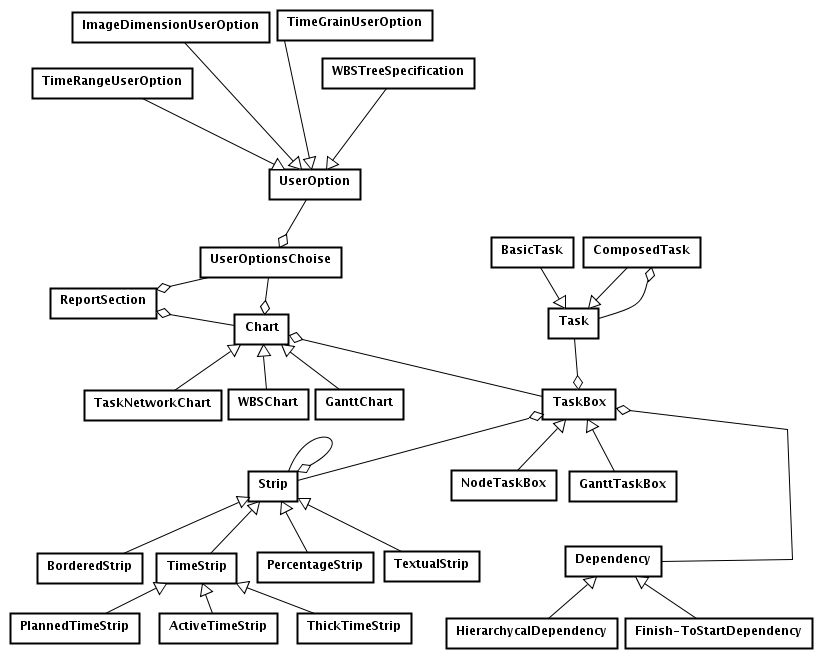
\includegraphics[width=1\textwidth]{../Milestone1-DomainModel/img/DomainModel.png}
	\caption{Overall UML diagram}
	\label{fig:overallDiagram} 
\end{figure}

Questo diagramma comprende tutti i concetti che abbiamo identificato durante la
prima iterazione del blocco di analisi. 

Nella figura abbiamo una visione di insieme che pu\`o essere utile a fini di
codifica e progettazione del piano delle prove. Finch\`e si rimane invece nella
sfera della progettazione (analisi inclusa) potrebbe produrre dei dubbi in
quanto propone molti concetti; mentre si sta cercando di raffinare le varie relazioni
secondo noi \`e necessaria una vista pi\`u in dettaglio di composizioni
di pochi concetti che sono legati tra loro, lasciando tutti gli altri ad una
loro commento separato.

Procediamo nel seguito del documento nella descrizione di piccole composizioni
in modo da chiarire i motivi per cui sono stati creati concetti e relazioni fra
essi.

\chapter{Aspects descriptions} 
% from here every document which is included with the input command must have a
% dedicated section whitin his body
\section{Task}
\label{sec:task}

\begin{figure}[h!] 
	\centering
	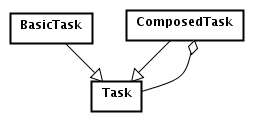
\includegraphics[width=0.4\textwidth]{../Milestone1-DomainModel/img/TaskDetail.png}
	\caption{task and its relations}
	\label{fig:task} 
\end{figure}

Molto probabilmente il concetto di \emph{Task} esiste gia nell'attuale
versione di \textbf{PMango 2.2.0}. Quello che abbiamo pensato \`e di introdurre
un \emph{glue layer} che ci permette di non apportare modifiche al codice
esistente di mango, ma lavorare con uno strato di intermezzo per essere il meno
intrusivi possibile e poter portare avanti il lavoro dipendendo solo dalle
nostri oggetti, facendo il minor riferimento al codice gia esistente.

Vogliamo rendere trasparente il concetto che un \emph{Task} sia un attivit\`a
singola (non scomponibile in sottoattivit\`a) che una attivit\`a scomposta. 

Costruiamo la relazione $\rightarrow$ che lega questi due concetti:
\begin{itemize}
  \item \emph{BasicTask} $\rightarrow$ attivit\`a di base, non ulteriormente
  scomponibili
  \item \emph{ComposedTask} $\rightarrow$ attivit\`a che sono composte da sotto
  attivit\`a
\end{itemize}
In questo modo possiamo trattare questi due tipi di attivit\`a in modo
interscambiabile e del tutto trasparente. Usando l'astrazione \emph{Task} non
ci importa se abbiamo una attivit\`a base o composta, in quanto cosi le abbiamo
portate ad avere interfaccie compatibili.

\section{TaskBox}
\label{sec:taskbox}

\begin{figure}[h!] 
	\centering
	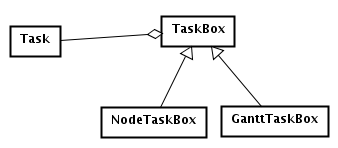
\includegraphics[width=0.5\textwidth]{../TaskBoxDetail.png}
	\caption{taskbox and its specializations}
	\label{fig:taskbox} 
\end{figure}

Il \emph{TaskBox} \`e la rappresentazione grafica di un
\emph{Task} (\autoref{fig:task}). Questo concetto astrae su queste
specializzazioni:
\begin{itemize}
\item \emph{GanttTaskBox} che ci permetter\`a di costruire la rappresentazione
in un \emph{GanttChart} conformi alle norme fissate nel documento di specifica.

\item \emph{NodeTaskBox} che ci permetter\`a di costruire la rappresentazione
in un \emph{WBSChart} e in \emph{TaskNetworkChart} alle norme fissate nel 
documento di specifica.
\end{itemize}

Abbiamo usato il principio di incapsulare il concetto che varia, modellando il
concetto astratto di \emph{TaskBox} per avere questi vantaggi:
\begin{itemize}
  \item non legare un \emph{Chart} specifico a una rappresentazione specifica
  \item aggiungere una nuova rappresentazione consiste nel modellarla e
  dichiarare che si tratta di una specializzazione di \emph{TaskBox}
  \item potremo cambiare a runtime il tipo di rappresentazione voluta nel
  disegno di un \emph{Chart}, magari inserire in un \emph{WBSChart} una
  rappresentazione pensata per i \emph{GanttChart}
\end{itemize}
\section{Strip}
\label{sec:strip}

\begin{figure}[h!] 
	\centering
	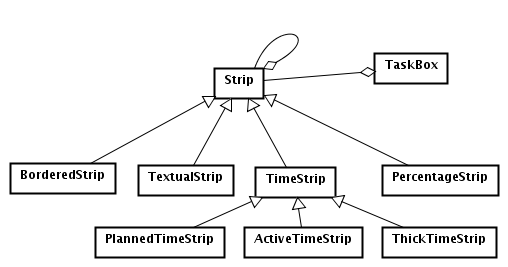
\includegraphics[width=0.7\textwidth]{../Milestone1-DomainModel/img/StripDetail.png}
	\caption{kinds of strips}
	\label{fig:strip} 
\end{figure}

La \emph{Strip} modella il concetto di ''striscia'': lo possiamo vedere come il
building block di pi\`u basso livello di tutta la nostra analisi. Si possono
osservare queste relazioni:
\begin{description}
  \item[TaskBox composition] \emph{TaskBox} contiene delle \emph{Strip},
  indipendentemente dalla rappresentazione dedicata ad uno specifico \emph{Chart}. Abbiamo costruito
  questa relazione in quanto per costruire un \emph{TaskBox} sar\`a sufficiente
  comporre un insieme di strip, tante quante sono necessarie per la corretta
  visualizzazione del \emph{Chart} che si sta disegnando.
  \item[russian doll] \emph{Strip} contiene a sua volta delle \emph{Strip}:
  questo \`e un concetto che pensiamo posso essere molto potente. Vogliamo rendere la
  \emph{Strip} un contenitore trasparente rispetto ad oggetti del suo stesso
  tipo. Questo ci permetter\`a di disegnare \emph{Strip} annidate, decidendo a
  runtime sia la \textbf{profondit\`a} di annidamento sia l'\textbf{ordine} con
  cui vengono annidate. Otteniamo cosi l'effetto di \emph{russian doll}, 
  dedicandoci a modellare solo alcune semplici specializzazioni di \emph{Strip},
  necessarie per l'implementazione delle notazioni richieste nel documento di specifica,
  limitandoci poi ad ottenere rappresentazioni complesse annidando quelle
  semplici.
  \item[specializations] abbiamo un primo livello di specializzazione:
  \begin{itemize}
    \item \emph{PercentageStrip} rappresenta un quantit\`a (l'intera
    \emph{Strip}) e la percentuale di comletamento (una parte di \emph{Strip}
    di colore diverso). Pu\`o essere composta da un \emph{GanttTaskBox} per
    indicare la percentuale di completamento relativa al \emph{Task}
    rappresentato.
    
    \item \emph{TextualStrip} permette di inserire delle stringhe di caratteri
    all'interno della \emph{Strip}. Questa possiamo utilizzarla ad esempio nel
    \emph{GanttChart} sulla destra della relativa \emph{TaskBox} per indicare
    l'effort oppure le risorse.
    
    \item \emph{BorderedStrip} permette di costruire un bordo, in modo che
    possiamo implementare la notazione per \emph{field} come richiesto per
    \emph{NodeTaskBox}
    
    \item \emph{TimeStrip} permettono di rappresentare informazioni relative a
    un intervallo di tempo. Queste sono i building blocks per
    \emph{GanttChart}. Possiamo specializzare ulteriormente questo concetto:
    \begin{itemize}
      \item \emph{PlannedTimeStrip} per costruire la parte superiore del
      \emph{GanttTaskBox} cdns
      \item \emph{ActualTimeStrip} per costruire la parte inferiore del
      \emph{GanttTaskBox} cdns      
      \item \emph{ThickTimeStrip} per costruire la parte superiore del
      \emph{GanttTaskBox} nel caso la rappresentazione sia di un
      \emph{ComposedTask} cdns
    \end{itemize}
  \end{itemize}
\end{description}

\section{Chart}
\label{sec:chart}

\begin{figure}[h!] 
	\centering
	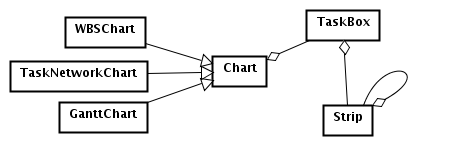
\includegraphics[width=0.6\textwidth]{../ChartDetail.png}
	\caption{chart and building blocks}
	\label{fig:chart} 
\end{figure}

Il \emph{Chart} modella il concetto di grafico generico. Per implementare la
specifica abbiamo queste specializzazioni:
\begin{itemize}
  \item \emph{GanttChart} che permette di avere la rappresentazione delle
  attivit\`a nel tempo
  \item \emph{WBSChart} per avere una vista gerarchica delle attivit\`a e di
  come sono state raffinate e decomposte in sotto attivit\`a
  \item \emph{TaskNetworkChart} per rappresentare le dipendenze di tipo
  \emph{finish-to start} fra coppie di attivit\`a
\end{itemize}

Per costruire un \emph{Chart} \`e sufficiente assemblare \emph{TaskBox} in base
ad alcune preferenze del client che richiede la generazione.

\section{Dependency}
\label{sec:dependency}

\begin{figure}[h!] 
	\centering
	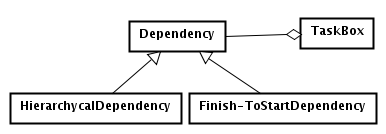
\includegraphics[width=0.5\textwidth]{../Milestone1-DomainModel/img/DependencyDetail.png}
	\caption{dependencies}
	\label{fig:dependencies} 
\end{figure}

\emph{Dependency} modella il tipo di dipendenze che possiamo rappresentare in
un \emph{Chart}. Per implementare la specifica abbiamo bisogno di incapsulare
queste varianti:\footnote{dire in quali Chart vengono utilizzate}
\begin{itemize}
  \item \emph{Finish-ToStartDependency}: siano $a, b$ due \emph{Task} tali
  che $b$ non pu\`o iniziare finch\'e $a$ non sia completato. Questa relazione
  \`e catturata da questa specializzazione.
  \item \emph{HierarchycalDependency}: siano $a, b_{i}$ con $i= 1,\ldots,n \in
  N$, \emph{Task}s tali che $a$ \`e scoposto in $b_{i}$ \emph{Task}. Questa
  relazione \`e catturata da questa specializzazione.
\end{itemize}
\section{UserOption}
\label{sec:userOption}

\begin{figure}[h!] 
	\centering
	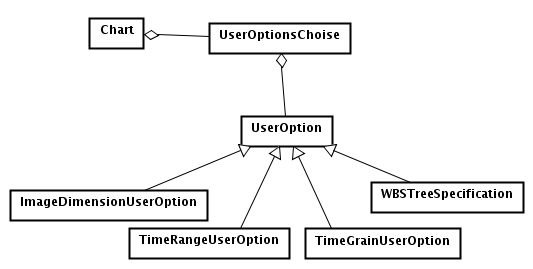
\includegraphics[width=0.7\textwidth]{../Milestone1-DomainModel/img/UserOptionDetail.png}
	\caption{UserOptions and choice}
	\label{fig:userOption} 
\end{figure}

Quando un generico client (potrebbe essere sia una persona fisica che un
oggetto astratto) della nostra implementazione della specifica vuole generare
un \emph{Chart} pu\`o guidare la generazione decidendo alcuni fattori che sono
di suo interesse. Questi fattori vengono modellati dal concetto di
\emph{UserOption}.

Ogni \emph{Chart} espone una lista di \emph{UserOption} per dare al client la
possibilit\`a di esprimere quali informazioni guidare. Questa lista varia da
\emph{Chart} a \emph{Chart}\footnote{creare un reference dove vengono mappate
questa relazione: potrebbe essere un appendici di questo documento??}.

Il concetto di lista di \emph{UserOption} \`e catturato in
\emph{UserOptionsChoice}.

Procediamo per passi: nelle prossime subsection osserviamo due aspetti che
trattarli insieme potrebbe non essere sufficiente per esporli in modo chiaro.

\subsection{\emph{UserOption}'s Instances}
\label{subsec:UserOptionInstances}
Questa \`e stata una decisione non molto facile da prendere. Il problema \`e
questo: nella specifica abbiamo che per ogni \emph{Chart} il committente ha
dichiarato quali \emph{UserOption} mostrare. Queste per\`o non rappresentano un
concetto che vogliamo catturare nel nostro modello, ma allo stesso tempo sono
\emph{istanze} (un insieme discreto quindi) di elementi che fissa il
committente.

Per questo motivo decidiamo di codificare questo insieme discreto in questo
documento e la successiva enumerazione \`e da considerarsi parte integrante del
diagramma inserito come figura.

Rappresentiamo il concetto espresso sopra indicando due descrizioni con questa
struttura di codifica:
\begin{itemize}
  \item \emph{istanze}, dove inseriamo tutte le possibili \emph{UserOption} che
  non possono essere ancora raffinate
  \item \emph{specializzazioni} dove inseriamo tutte le possibili
  specializzazioni di \emph{UserOption} che possono essere ancora raffinate,
  ripetendo in modo ricorsivo questa struttura di codifica
\end{itemize}

Le successive descrizioni sono relative al concetto di \emph{UserOption}:
\begin{description}
  \item[istanze]\footnote{inserire qui la il mapping sui vari Chart?}
  \emph{WBSExplosionLevelUserOption, ActualTimeFrameOption, CompletitionBarOption, \\ PlannedDataOption, ActualDataOption,
  AlertMarkUserOption, ReplicateArrowUserOption, FindCriticalPathUserOption,
  WBSUserSpecificationUserLevel, \\WBSUserSpecificationUserLevel,
  ResourcesDetailsOption, TaskNameOption, CompleteDiagramUserOptions,
  ShowDependencies}
  \item[specializzazioni] \quad
  \begin{itemize}
    \item \emph{WBSTreeSpecification}
    \begin{description}
  \item[istanze] \emph{LevelSpecification, UserCustomSpecification}
  \item[specializzazioni] nessuna
\end{description}

\item \emph{TimeGrainUserOption}
    \begin{description}
  \item[istanze] \emph{HourlyGrain, DailyGrain, WeaklyGrain, MonthlyGrain,
  AnnuallyGrain}
  \item[specializzazioni] nessuna
\end{description}

\item \emph{ImageDimensionUserOption}
    \begin{description}
  \item[istanze] \emph{CustomDim, FitInWindowDim, OptionalDim, DefaultDim}
  \item[specializzazioni] nessuna
\end{description}

\item \emph{TimeRangeUserOption}
    \begin{description}
  \item[istanze] \emph{CustomRange, WholeProjectRange, FromStartRange, ToEndRange}
  \item[specializzazioni] nessuna
\end{description}

  \end{itemize}
\end{description}

\subsection{\emph{UserOptionsChoice}}
Questo concetto \`e, secondo la nostra analisi, molto importante in quanto ci
permette di astrarre dal client che richiede una generazione.

Il motivo per cui abbiamo introdotto questo concetto \`e di poter lavorare lato
server usando \emph{UserOptionsChoice} per controllare quali informazioni il
client vuole guidare. In questo modo non siamo vincolati ad accedere ai dati
inviati per \emph{POST, GET} dalla form HTML, ma possiamo direttamente guardare
in \emph{UserOptionsChoice}. Queste ci permette di disaccopiare il processo di
generazione della maschera di input di una pagina HTML. 

Se vogliamo utilizzare il processo di generazione (che comunque \`e
server side) scrivendo un programma client (GUI o da riga di comando) che
costruisce una HTML request ad hoc (dovremo definire una grammatica e
attribuire la semantica ai contesti, questo \`e necessario, non ch\`e scrivere 
un parser), usando \emph{UserOptionsChoice} e il suo disaccoppiamento ci sar\`a
possibile farlo. 

Una volta ricevuta la response possiamo maneggiare la pagina
inviata come una response HTML valida e usarla per i nostri obiettivi (possiamo
rihiedere l'immagina generata, o il file PDF generato, salvandolo in
locale, oppure visualizzando lo stesso con un browser, ma possiamo anche
inserire in un db oppure farci dei test sopra\ldots).

Dovremo quindi costruire un oggetto che si incarica di costruire
\emph{UserOptionsChoice} in base al tipo di richiesta ricevuta (da una pagina
html come \`e il caso di PMango, oppure una richiesta da un client indipendente
scritto in un qualche linguaggio). Una volta costruito l'insieme delle
\emph{UserOption} \`e possibile iniziare la generazione. Questo sar\`a delegato
alla fase di progettazione.

\section{ReportSection}
\label{sec:reportSection}

\begin{figure}[h!] 
	\centering
	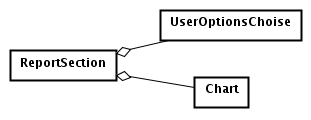
\includegraphics[width=0.5\textwidth]{../ReportSectionDetail.png}
	\caption{report section}
	\label{fig:reportSection} 
\end{figure}

Abbiamo da implemetare un requisito che vuole la possibilit\`a di aggiungere
alla reportistica un determinato \emph{Chart} con le relative \emph{UserOption}
scelte dall'utente. Modelliamo quindi il concetto di \emph{ReportSection} per
realizzare questo requisito. Come si vede dalla figura, \emph{ReportSection}
associa \emph{Chart} e \emph{UserOptionChoice}. Utilizziamo direttamente la
lista delle scelte\footnote{che viene costruita lato server} in modo da non
doverla costruire nella funzionalit\`a di assemblamento del report.



\part{Use cases}

\documentclass[a4paper, 12pt]{report}

\usepackage{charter}
\usepackage{makeidx}
\usepackage{fancyhdr}
\usepackage{hyperref}
\usepackage[utf8]{inputenc}
\usepackage{graphicx}
\usepackage[left=2cm, right=2cm]{geometry}
\usepackage{latexsym}
\usepackage{amsmath, amsthm, amssymb}
\usepackage{rotating}


\begin{titlepage}
\title{Use cases}
\author{Release 0.8}
\date{\today \\Firenze \\\begin{figure}[h] \centering

\includegraphics[width=0.2\textwidth]{../../images/logokiwi.png} \end{figure} }
\end{titlepage}

\pagestyle{fancy}

\begin{document}

\maketitle

\section*{Approvazione, redazione, lista distribuzione}
\begin{table}[h!]
  \begin{center}
    \begin{tabular}{| l | l | p{60mm} |}
    \hline
    \textbf{approvato da} & \textbf{il giorno} & \textbf{firma} \\
	\hline    
	Marco Tinacci &  &  \\
    \hline
    \end{tabular}
  \end{center}
\end{table}

\begin{table}[h!]
  \begin{center}
    \begin{tabular}{| l | l | p{60mm} |}
    \hline
    \textbf{redatto da} & \textbf{il giorno} & \textbf{firma} \\
    \hline
    Francesco Calabri &  &  \\
    \hline
	Manuele Paulantonio &  &  \\
    \hline    
	Massimo Nocentini &  &  \\
    \hline
    \end{tabular}
  \end{center}
\end{table}

\begin{table}[h!]
  \begin{center}
    \begin{tabular}{| l | l | p{60mm} |}
    \hline
    \textbf{distribuito a} & \textbf{il giorno} & \textbf{firma} \\
	\hline    
	Daniele Poggi &  &  \\
    \hline
	Niccol\'o Rogai &  &  \\
    \hline
	Marco Tinacci &  &  \\
    \hline
    \end{tabular}
  \end{center}
\end{table}

\tableofcontents

\newpage

\section*{Introduzione}
Descrizione dell'acronimo: \textbf{cdns} sta per ''\textbf{c}ome
\textbf{d}escritto \textbf{n}ella \textbf{s}pecifica''.

\chapter*{Entire System UML diagram}
\begin{figure}[h!] \centering
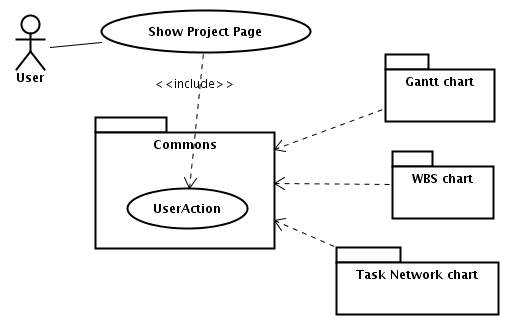
\includegraphics[width=0.7\textwidth]{EntireSystem.png} 
\caption{Entire system UML diagram}
\label{fig:entireSystemDiagram}
\end{figure}

\chapter{Commons}
\begin{figure}[h!] \centering
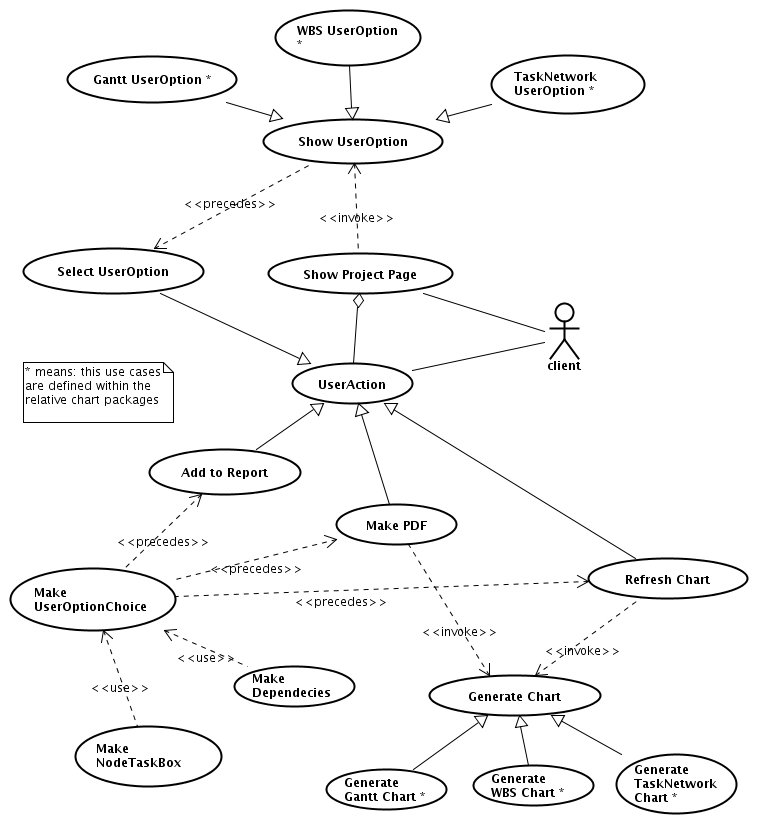
\includegraphics[width=0.9\textwidth]{Commons/img/Overall.png} 
\caption{Overall Commons UML diagram}
\label{fig:commonsOverallDiagram}
\end{figure}

\section{Make Dependencies}
\label{seq:makeDependencies}
\subsection{Basic course}
Si assume che l'insieme di \emph{TaskBox} sia gi\`a costruito.\\\\
Il client richiede di rappresentare graficamente le
\emph{Finish-ToStartDependency} relative all'insieme di \emph{TaskBox} gi\`a
costruite.

Il sistema esegue questi passi:
\begin{enumerate}
  \item costruisce un insieme $Dep$ di coppie del tipo $(a,b)$, con $a,b \in
  $\emph{TaskBox}, tale che $(a,b) \in Dep \Leftrightarrow b$ non pu\`o
  iniziare finch\`e $a$ non \`e stata completata.
  \item per ogni coppia $(a,b) \in Dep$ costruisci una linea
  spezzata cdns.
\end{enumerate}

\subsection{Alternative course}
\begin{description}
\item[not well formed project] Se la struttura al albero WBS del progetto non
\`e ben formata allora si deve cercare di dare la migliore euristica possibile
per la rappresentazione delle dipendenze.

\end{description}
\section{Make NodeTaskbox}
\label{seq:makeNodeTaskbox}
\subsection{Basic course}
Il client prende un reference al \emph{WBSChartGenerator} e domanda di creare la
rappresentazione grafica di un \emph{Task}.

Il sistema esegue questi passi:
\begin{enumerate}
  \item recupera il \emph{Task} da rappresentare.
  \item costruisce la rappresentazione grafica, il \emph{NodeTaskbox}
    in base alla scelta \emph{WBSTreeSpecification}. Il \emph{NodeTaskbox} \`e
    una composizione di \emph{Strip}. Il sistema costruisce una
    biezione tra \emph{BoxedStrip} e le scelte presenti in 
    \emph{UserOptionsChoice} in questo modo:
    \begin{itemize}
      % task name
      \item se \emph{UserOptionsChoice} contiene
      \emph{TaskNameOption}, allora costruisce una
      \emph{Strip} contenente il nome del \emph{Task} cdns.
      
      % resources
   	  \item se \emph{UserOptionsChoice} contiene \emph{ResourcesDetailsOption},
    	allora sul margine destro della \emph{GanttTaskBox} appendi la stringa
    	contenente la lista delle risorse cdns.
    	
    	Altrimenti appendi sul margine destro l'effort cdns.
      
      % planned time frame
      \item	se \emph{UserOptionsChoice} contiene \emph{PlannedTimeFrameOption} 
     allora costruisce due \emph{Strip} adiacenti contenenti rispettivamente le
     date di inizio e fine \emph{Task} cdns.
    	
	  % actual time frame
    	\item se \emph{UserOptionsChoice} contiene \emph{ActualTimeFrameOption}
    	allora costruisce due \emph{Strip} adiacenti contenenti rispettivamente 
    	le date di inizio e fine \emph{Task} reali cdns.
    	
		% planned data
    	\item se \emph{UserOptionsChoice} contiene \emph{PlannedDataOption} allora
    	costruisce tre \emph{Strip} adiacenti contenenti rispettivamente la durata
    	pianificata, lo sforzo complessivo pianificato, il costo
    	pianificato del \emph{Task} cdns.
    	
    	%actual data
    	\item se \emph{UserOptionsChoice} contiene \emph{ActualDataOption} allora
    	costruisce tre \emph{Strip} adiacenti contenenti rispettivamente la durata
    	“dall’inizio ad oggi”, lo sforzo complessivo “ad oggi” effettuato, il
    	costo complessivo “ad oggi” del \emph{Task} cdns.
    	
    	% completition bar
		\item se \emph{UserOptionsChoice} contiene \emph{CompletitionBarOption}
		allora costruisce la barra di completamento del \emph{Task} cdns.
		
		\item to complete with the missing options
		
    \end{itemize}
\end{enumerate}

\subsection{Alternative course}
\begin{description}
  \item[troncamento del nome del \emph{Task}] se la stringa scritta supera la
  dimensione fissata nel documento di specifica, allora il sistema la tronca
  cdns.


\end{description}

\section{Show Project Page}
\label{seq:showProjectPage}
\subsection{Basic course}
Il client digita l'URL della \emph{ProjectPage}\footnote{TODO:definire
ProjectPage nel documento dei Mockup}. \\
Il sistema invia in risposta la pagina richiesta aggiungendo all'insieme dei
tab presenti, tre tab relativi ai \emph{Chart} descritti nel documento
\textbf{Domain Model} e oggetto dell'appalto.\\
Il client fa click sul tab relativo al \emph{Chart} che vuole generare.\\
Il sistema invoca la specializzazione dello usecase \ref{seq:showUserOptions}
relativa al \emph{Chart} scelto, per costruire l'insieme delle possibili
\emph{UserOption}: dopo di che aggiunge questo insieme alla pagina di
risposta.\\
Il client effettua una azione, invocando una specializzazione di
\ref{seq:userAction}.
\section{Generate Chart}
\label{seq:generateChart}
Questo use case, come rappresentato nel diagramma UML
\autoref{fig:commonsOverallDiagram}, fornisce il punto di astrazione per altri
use case. Per questo motivo la descrizione del comportamento che  si
vuole modellare viene descritta in ogni specializzazione.
\section{Show UserOptions}
\label{seq:showUserOptions}
\subsection{Basic course}
Il client digita l'URL della \emph{ProjectPage}\footnote{TODO:definire
ProjectPage nel documento dei Mockup}. 

Il sistema invia in risposta la pagina richiesta con i tre tab relativi ai
\emph{Chart} descritti nel documento \textbf{Domain Model}. 

Il client fa click sul tab relativo al \emph{Chart} che vuole visualizzare.

Il sistema costruisce il contenuto del tab inserendo una sequenza di
\emph{UserOption}. 

Il client esegue la sua selezione delle informazioni che
vuole visualizzare nel \emph{Chart} e clicca su un oggetto\footnote{come posso
speficare questo oggetto?} per domandare la generazione del \emph{Chart}.

Il sistema esegue questi passi:
\begin{enumerate}
  \item costruisce \emph{UserOptionsChoice} in base alle opzioni selezionate
  dal client.
  \item recupera i \emph{Task} da includere nel \emph{Chart}.
  \item esegue la generazione\footnote{dire che la generazione astrae sui
  formati: la richiesta potrebbe essere o la visualizzazione della gif nel
  browser come attualmente fa mango, altrimenti la richiesta di generazione
  pdf. Inserire questo paragrafo come un description sotto il punto a cui
  appartiene questa nota.}
\end{enumerate}

\subsection{Alternative course}
\begin{description}
\item[Nessuna \emph{UserOption} selezionata] Il client invia un request con 
selezione delle \emph{UserOption} vuota. Quindi il sistema genera il
\emph{Chart} con delle \emph{UserOption} di default\footnote{dedicare un
paragrafo in un qualche documento per definire quali sono le opzioni di
default per ciascun chart.}.
\end{description}
\section{Make UserOptionsChoice}
\label{seq:makeUserOptionsChoice}
\subsection{Basic course}
Il sistema riceve una http request contenente una sequenza di \emph{UserOption}
che sono state selezionate dall'utente. Costruisce una
\emph{UserOptionsChoice} cosi: per ogni \emph{UserOption} indicata nella
request si aggiunge all'oggetto in costruzione.

Lato server abbiamo l'insieme di scelte disponibile per le azioni successive.
\section{User Action}
\label{seq:userAction}
Questo use case, come rappresentato nel diagramma UML
\autoref{fig:commonsOverallDiagram}, fornisce il punto di astrazione per altri
use case. Per questo motivo la descrizione del comportamento che  si
vuole modellare viene descritta in ogni specializzazione.
\section{Add to Report UserAction}
\label{seq:addToReportUserAction}
\subsection{Basic course}
Si assume che il client stia interagendo con il tab relativo al \emph{Chart}
che vuole generare.

Il client fa click sul pulsante ``Add to Report''.\\
Il sistema invoca lo use case \ref{seq:makeUserOptionsChoice} per costruirsi la
\emph{UserOptionsChoice}. \\
Il sistema aggiunge una \emph{ReportSection} per aggiungere alla reportistica
il \emph{Chart} richiesto, con la relativa \emph{UserOptionsChoice}. Queste
sezioni saranno elencate nella schermata della reportistica gi\`a esistente.
\section{Make PDF}
\label{seq:GanttMakePDF}

\subsection{Basic course}
Il client entra nella pagina relativa al diagramma Gantt e clicca sulla 
funzionalit\`a ''Make PDF''. Il sistema costruisce un oggetto in questo modo:
\begin{itemize}
  \item invoca lo use case \ref{seq:GanttMakeLeftColumn} per creare la
  colonna a sinistra.
  \item invoca lo use case \ref{seq:GanttRightRepresentation} per creare
  la rappresentazione nel tempo (colonna destra del diagramma).
\end{itemize}
Il sistema invio la pagina di risposta al client, aggiungendo accanto ai
pulsanti di reporting una icona per permettere il download del file generato.  

\subsection{Alternative course}
\begin{description}
\item[nessuna]
\end{description}


\section{Refresh Chart}
\label{seq:refreshChart}
\subsection{Basic course}
Si assume che il client stia interagendo con il tab relativo al \emph{Chart}
che vuole generare.

Il client fa click sul pulsante ``Refresh''.\\
Il sistema esegue questi passi:
\begin{itemize}
  \item invoca lo use case \ref{seq:makeUserOptionsChoice} per costruirsi la
  \emph{UserOptionsChoice}.
  \item esegue una ricerca dei \emph{Task} che devono essere inclusi nel
  \emph{Chart}.  
  \item invoca la specializzazione di \ref{seq:generateChart} per la
  creazione del relativo \emph{Chart}
  \item invia al client una pagina di risposta inserendo la rappresentazione
  nel bottom della pagina.
\end{itemize}
\section{Select User Option}
\label{seq:selectUserOption}
\subsection{Basic course}
Si assume che il client stia interagendo con il tab relativo al \emph{Chart}
che vuole generare, quindi lo use case \ref{seq:showProjectPage} \`e gi\`a
stato completato. \\\\
Il client vuole selezionare alcune \emph{UserOption} per guidare la
rappresentazione delle informazioni che verranno codificate nel \emph{Chart}.\\
Queste sono rappresentate tramite una form html, sotto forma di controlli
grafici, dipendenti dal tipo e dalla semantica della \emph{UserOption} che
rappresentano. \footnote{inserire qua il mappaggio tra il tipo di UserOption e
il controllo grafico che viene bindato.}
Il sistema non effettua alcuna azione in quanto il fatto di memorizzare le
scelte fino al ``submit'' viene tenuto dalla form html stessa.


\chapter{Gantt chart}
\section*{Overall UML diagram}
\begin{figure}[h!] \centering
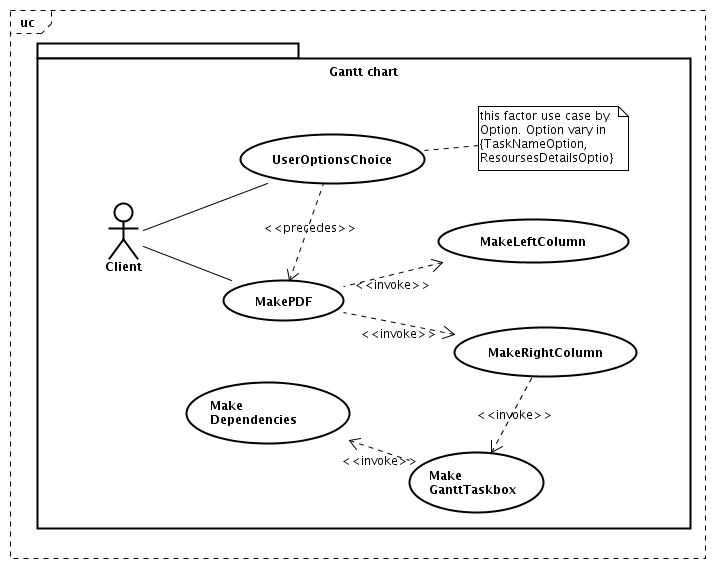
\includegraphics[width=0.8\textwidth]{Gantt/img/GanttChart.png} 
\caption{Gantt Overall UML diagram}
\label{fig:ganttDiagram}
\end{figure}

\section{Make Left Column}
\label{seq:GanttMakeLeftColumn}
\subsection{Basic course}
Il client prende un reference al GanttChartGenerator e domanda la funzionalit\'a
per creare la colonna di sinistra del diagramma. \\
Il sistema costruisce una colonna di larghezza di dimensione \emph{fissa}.
Guarda se in UserOptionChoises \`e presente l'opzione TaskNameOption:
\begin{itemize}
  \item se \'e presente allora calcola la larghezza
\begin{displaymath}
	width_{nor}=lenght(max\lbrace id | \forall task: id =
WBS\_identifier(task) \rbrace) 
\end{displaymath}
dove la funzione $WBS\_identifier$ restituisce il WBS identifier relativo al 
parametro $task$ del dominio.

Poi $\forall task$ scrive $WBS\_identifier(task)$, un task per ogni riga.

\item altrimenti calcola
\begin{eqnarray}
width_{opt}=lenght(max\lbrace ::(id, task\_name) | \forall task: \\ id =
WBS\_identifier(task), \\ task\_name = Get\_TaskName(task)
\rbrace)
\end{eqnarray}
dove l'operatore $::$ concatena le stringhe passate come parametro, e
l'operatore \\$Get\_TaskName$ restituisce il nome del parametro
task.

Poi $\forall task$ scrive $::(WBS\_identifier(task), Get\_TaskName(task)$, un
task per ogni riga.
\end{itemize}

\subsection{Alternative course}
\begin{description}
\item[troncamento delle resourses] se $width_{opt} >
\frac{width_{diagram}}{6}$, con $width_{diagram}$ uguale alla larghezza totale
del diagramma, allora sia 
\begin{equation}cutted = cut(::(WBS\_identifier(task),
Get\_TaskName(task))\end{equation} 
la funzione $cut$ cancella caratteri in coda alla stringa in ingresso e
restituisce $cutted$, contenente i caratteri non cancellati, in modo che $cutted
= \frac{width_{diagram}}{6}-3$. \\ Il sistema scrive 
\begin{equation} 
::(cut(::(WBS\_identifier(task), Get\_TaskName(task)), ''\ldots'')
\end{equation}
\item[troncamento del WBS identifier] se avessi un identifier troppo lungo
dovrei fare lo stesso??
\end{description}
\section{Make GanttTaskbox}
\label{seq:makeGanttTaskbox}
\subsection{Basic course}
Il client prende un reference al GanttChartGenerator e domanda di creare la
rappresentazione grafica di un \emph{Task}. 

Il sistema esegue questi passi:
\begin{enumerate}
  \item recupera il \emph{Task} da rappresentare
  \item costruisce la rappresentazione grafica, il \emph{GanttTaskBox}
    in base alla scelta \emph{WBSTreeSpecification}.
  \item \`E possibile codificare delle informazioni aggiuntive:
    \begin{itemize}
   	  \item se \emph{UserOptionChoice} contiene \emph{ResourcesDetailsOption},
    	allora sul margine destro della \emph{GanttTaskBox} appendi la stringa
    	contenente la lista delle risorse cdns.
    	
    	Altrimenti appendi sul margine destro l'effort cdns.
    \end{itemize}
    
\end{enumerate}

\subsection{Alternative course}
\begin{description}
\item[troncamento delle resourses] se le informazioni testuali aggiuntive
superano la dimensione definita nel documento di specifica, allora si troncano
cdns.

\end{description}
\section{Make Right Column}
\label{seq:GanttRightRepresentation}
\subsection{Basic course}
Il client prende un reference al GanttChartGenerator e domanda di creare la
colonna di destra del diagramma. 

Il sistema esegue questi passi:
\begin{enumerate}
  \item costruisce una colonna di larghezza di dimensione \emph{fissa} che
  viene calcolata cdns.
  \item Il sistema effettua una ricerca per calcolare l'insieme dei \emph{Task}
  necessari da rappresentare nella colonna.
  \item Per ogni \emph{Task} trovato:
  \begin{itemize}
    \item invoca lo use case \ref{seq:makeGanttTaskbox}
    
    \item si posiziona il \emph{GanttTaskBox} creato nella giusta posizione
    temporale in base alla scelta \emph{TimeGrainOption}.
  \end{itemize}
  \item se \emph{UserOptionsChoice} contiene \emph{ShowDependencies} allora per
  ogni \emph{TaskBox} rappresentata, invoca lo use case 
  \ref{seq:makeDependencies}
\end{enumerate}

\subsection{Alternative course}
\begin{description}
\item[troncamento delle resourses] se le informazioni testuali aggiuntive
superano la dimensione definita nel documento di specifica, allora si troncano
cdns.

\end{description}
\section{Make PDF}
\label{seq:GanttMakePDF}

\subsection{Basic course}
Il client entra nella pagina relativa al diagramma Gantt e clicca sulla 
funzionalit\`a ''Make PDF''. Il sistema costruisce un oggetto in questo modo:
\begin{itemize}
  \item invoca lo use case \ref{seq:GanttMakeLeftColumn} per creare la
  colonna a sinistra.
  \item invoca lo use case \ref{seq:GanttRightRepresentation} per creare
  la rappresentazione nel tempo (colonna destra del diagramma).
\end{itemize}
Il sistema invio la pagina di risposta al client, aggiungendo accanto ai
pulsanti di reporting una icona per permettere il download del file generato.  

\subsection{Alternative course}
\begin{description}
\item[nessuna]
\end{description}



\chapter{WBS chart}
\section*{Overall UML diagram}
\begin{figure}[h!] \centering
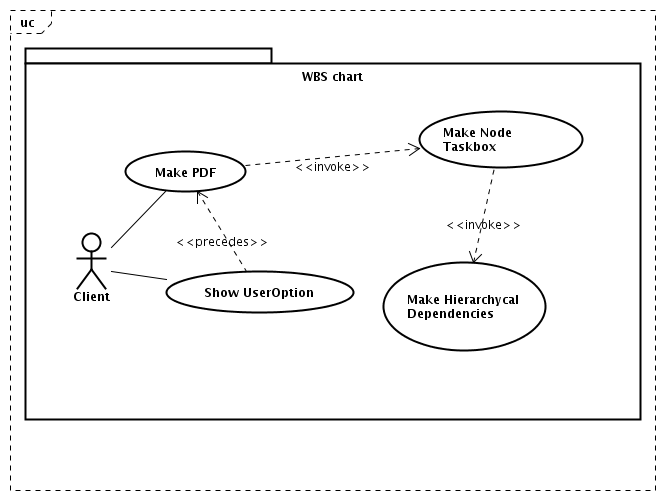
\includegraphics[width=0.8\textwidth]{WBS/WBSChart.png}
\caption{WBS UML diagram}
\label{fig:WBSdiagram}
\end{figure}

\section{Make Hierarchycal Dependencies}
\label{seq:makeHierarchycalDependencies}
\subsection{Basic course}
Il client richiede la funzionalità di rappresentazione della relazione 
gerarchica di un task.

Il sistema esegue questi passi:
\begin{enumerate}
  \item in base alle informazioni in \emph{WBSTreeSpecification}, recupera i
  figli del task (non l’intera discendenza, solo quelli di livello successivo) e
  li dispone graficamente al di sotto di esso.
  \item La distanze fra livelli e tra taskbox appartenenti allo stesso
  livello rispettano queste regole:
  \begin{itemize}
    \item la distanza \emph{inter-Taskbox} fra coppie di
    \emph{Taskbox} adiacenti, rappresentati sullo stesso livello, deve essere
    equa ed uguale per ogni coppia (questa regola si ripete in modo iterativo
    per ogni coppia appartenente ad un livello $l$)
	\item la distanza \emph{inter-Level} fra coppie di livelli contenenti le 
	rappresentazioni dei task padre e i suoi figli deve essere equa e uguale
	per ogni coppia di livelli (questa regola si applica ricorsivamente al livello
	dei figli, nel caso che almeno un figlio sia composto da subtask)
  \end{itemize} 
  
  \item Il sistema collega il task ai suoi figli con linee spezzate cdns.
\end{enumerate}

\subsection{Alternative course}
\begin{description}
\item[WBSExplosionLevel = 0] se il livello di visualizzazione della WBSStructure
richiesto si limita alla root, crea il solo un \emph{NodeTaskbox} rappresentante
l’intero progetto.
\end{description}


\section{Make PDF}
\label{seq:GanttMakePDF}

\subsection{Basic course}
Il client entra nella pagina relativa al diagramma Gantt e clicca sulla 
funzionalit\`a ''Make PDF''. Il sistema costruisce un oggetto in questo modo:
\begin{itemize}
  \item invoca lo use case \ref{seq:GanttMakeLeftColumn} per creare la
  colonna a sinistra.
  \item invoca lo use case \ref{seq:GanttRightRepresentation} per creare
  la rappresentazione nel tempo (colonna destra del diagramma).
\end{itemize}
Il sistema invio la pagina di risposta al client, aggiungendo accanto ai
pulsanti di reporting una icona per permettere il download del file generato.  

\subsection{Alternative course}
\begin{description}
\item[nessuna]
\end{description}



\end{document}

\part{Mockups}

\chapter*{Release \textbf{1.0}}

\chapter{Gantt chart}

\begin{sidewaysfigure}[h!] 
\centering
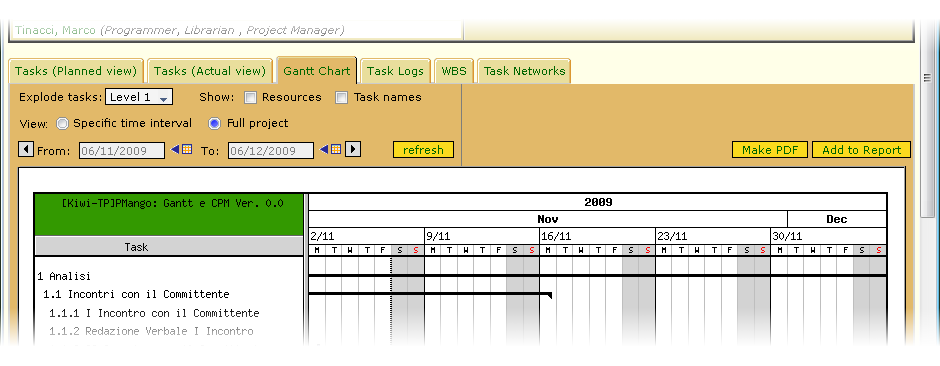
\includegraphics[width=1\textwidth]{../Mockup/Gantt.png}
\caption{Gantt tab mockup}
\end{sidewaysfigure}

\chapter{WBS chart}

\begin{sidewaysfigure}[h!] 
\centering
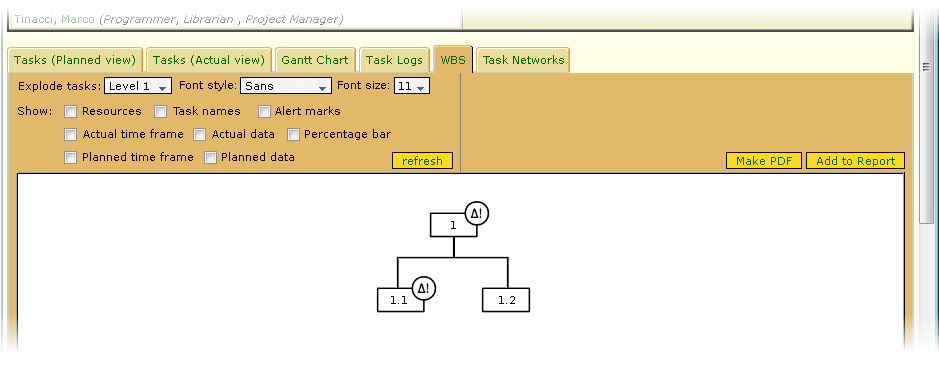
\includegraphics[width=1\textwidth]{../Mockup/WBS.png}
\caption{WBS tab mockup}
\end{sidewaysfigure}

\chapter{Task Network chart}

\begin{sidewaysfigure}[h!] 
\centering
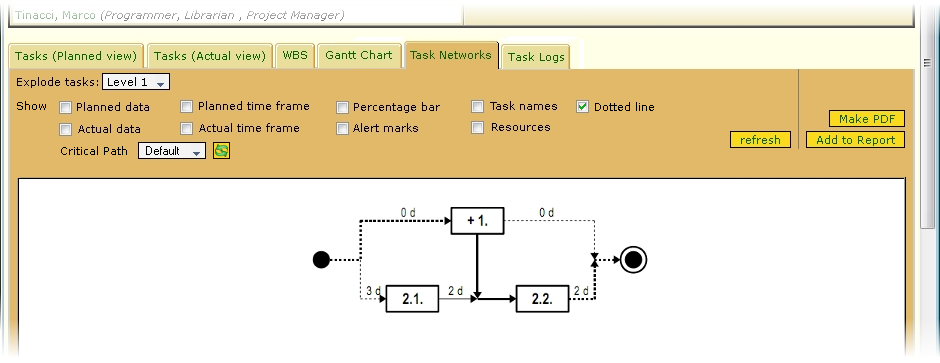
\includegraphics[width=1\textwidth]{../Mockup/TN.png}
\caption{Task Network tab mockup}
\end{sidewaysfigure}

\end{document}